\documentclass[10pt]{beamer}

\usetheme[progressbar=frametitle]{metropolis}
\usepackage{appendixnumberbeamer}

\usepackage{booktabs}
\usepackage[scale=2]{ccicons}

\usepackage{pgfplots}
\usepgfplotslibrary{dateplot}
\usepackage{verbatim}
\usepackage{xspace}
\newcommand{\themename}{\textbf{\textsc{metropolis}}\xspace}

\title{The welfare effects of vertical integration in multichannel television markets}
\subtitle{}
 \date{\today}
%\date{}
\author{Hao GENG}
\institute{Department of Economics,CUHK}
 \titlegraphic{\hfill\includegraphics[height=1.5cm]{}}

\begin{document}

\maketitle

\begin{frame}{Table of contents}
  \setbeamertemplate{section in toc}[sections numbered]
  \tableofcontents[hideallsubsections]
\end{frame}

\section{Introduction}

\begin{frame}[fragile]{What others do}
.   \begin{itemize}
    \item important and controversial
    \item theoretical pro anti-competitive impacts of vertical integration is vast, elimination of double marginalization, alighment of investment incentives.
    \item empirical, quantitative magnitudes of these potential effects; the overall net welfare effect.
\end{itemize}
\end{frame}
\begin{frame}[fragile]{what we do}
    \begin{itemize}
        \item this paper quantifies the welfare effects of vertical integration in cable and satellite television in the context of high-value regional sports programming in the United States market.
        \item whether the ownership of content by distributors harms welfare
        \item the industry is big and influential.
        \item \textbf{our focus on the multichannel television industry and in particular regional sports programming is driven by several factors that create empirical leverage to adddress this question.} 
        \item first, variation in terms of ownership of regional sports content by cable and satelite distributors, that is , multichannel video programming distributors (MVPDs). 
        \item variation in ownership patterns both across region and time ,regional sports networks.
        \item third, the industry is under regulatory and antitrust attention in addition to merger review; the application of "program access rules" and exceptions to this rule.
    \end{itemize}
\end{frame}
\begin{frame}{What we do 2}
    \begin{itemize}
        \item two key components:comprehensive data and the specification and estimation of a structural model of the multichannel industry that captures consumer viewership and subscription decisions, MVPD pricing and carriage decisions and bargaining between MVPDs and content providers.
        \item An important input identifying these effects is our estimates of the change in distributor profits from the addition or removal of an RSN from any of its programming bundles.
        
    \end{itemize}
\end{frame}
\begin{frame}{Related Literature}
    \begin{itemize}
        \item Previous studies on cable industry: reduced-form cross-sectional limited subset of channels.
        \item Could not separate efficiency from foreclosure incentives
        \item could not make welfare statements
        \item We complement 1. structural model to make welfare statements and identify the mechanisms.
        \item 2. richer panel data set on consumer viewership and bundle subscription and the pricing carriage and bargaining decisions. 
        \item 
    \end{itemize}
    
\end{frame}

\begin{frame}{Challenges}
    \begin{itemize}
        \item pollution and price are likely to be endogenous.
        \item spatial regression discontinuity by using Huai River policy in heating supply.
        \item first, product FE and city FE
        \item for product-city level unobserved variables, IV: distance from manufacturing location (import port) to city.
    \end{itemize}
\end{frame}
\begin{frame}{Main Results}
    \begin{itemize}
        \item air pollution is discontinuously higher in cities north.
        \item market share is higher in the north discontinuously.
        \item WTP for removing the amount of PM10 generated by the Huai River policy for five years is USD 190.
        \item MWTP removing 1 ug/m3 for five years is 4.4 usd.
        \item distribution of WTP:BLP. Higher income has higher MWTP.
    \end{itemize}
\end{frame}

\begin{frame}{Contributions}
    \begin{itemize}
        \item we develop a framework to estimate WTP on clean air based on defensive investment
        \item policy implications.
        \item empirical evidence of an important missing piece in the literature of air pollution in developing countries.
    \end{itemize}
\end{frame}

\section{Institutional Detail and Data}
\begin{frame}{Summary Statistics}
    \begin{columns}[c] 
    \column{9cm}
    \begin{figure}
        \centering
        \includegraphics[height=8cm]{table1}
    \end{figure}
    \column{4cm}
    \begin{itemize}
        \item Air purifier,air pullution,manufacturing/importing location data for each j (IV),demographic info (2005 Census)
        \item air purifier:2006.1-2012.12,81 cities. \ org:product-city-store-y-m after:product-city.
        \item pollution data:
        \item demographics: 
    \end{itemize}
	\end{columns}
\end{frame}

\section{Model}
\begin{frame}{3.1 Notations and model settings}
    \begin{itemize}
        \item $i$:consumer,$m$:market,$t$:time.
        \item set of downstream video programming distributors (MVPDs):$\mathcal{F}_{t}$;
        \item set of upstream channels $\mathcal{C}_t$ active in each period t.
        \item $\mathcal{F}_{mt}$
        \item assume each MVPD $f \in \mathcal{F}_{mt}$ offers a single bundle of channels $\mathcal{B}_{fmt} \subset \mathcal{C}_t$ in market m and time t, where a household subscribing to this bundle pays a price $p_{fmt}$ and have access to all channels $c \in \mathcal{B}_{fmt}$
        \item in each period (year), stage 1: channels and distributors bargin bilaterally to decide afiliate fees and distributors set prices and make carriage decisions for each market they operate.
        \item stage 2: household choose which MVPD or 0 to subscribe to in their market; stage 3: consumers view televison channels.
    \end{itemize}
\end{frame}

\begin{frame}{3.2 stage 3: household viewing}
    \begin{itemize}
        \item $u_{ijc}=\beta_{i}x_{jc}+\alpha_{i}p_{jc}+\eta_j+\lambda_c+\xi_{jc}+\epsilon_{ijc}$ (1)
        \item $\beta_i=\beta$,$\alpha_i=\alpha$
        \item $s_{jc}=\frac{exp(\beta x_{jc}+\alpha p_{jc}+\eta_j+\lambda_c+\xi_{jc})}{\sum_{k=0}^J exp(exp(\beta x_{kc}+\alpha p_{kc}+\eta_k+\lambda_c+\xi_{kc})}$ (2)
        \item outside good:j=0 not to buy.
        \item assume potential buyers are number of households in c, buy either one or zero.\
        $x_{0c}=0$
        \item $lns{0c} = -ln(\sum_{k=0}^J exp(exp(\beta x_{kc}+\alpha p_{kc}+\eta_k+\lambda_c+\xi_{kc}))$ ?
        \item $lns_{jc}-lns_{0c}=\beta x_{jc}+\alpha p_{jc}+\eta_j+\lambda_c+\xi_{jc}$ (3)
        \item $-\beta/\alpha$:marginal utility for clean air/marginal utility from price. Marginal WTP(MWTP).
    \end{itemize}
\end{frame}

\begin{frame}{stage 2}
    \begin{itemize}
        \item $u_{ifmt}=\beta^{v}v^{*}_{ifmt}+\boldsbeta^{x}\boldsymbol{x}_{fmt}+\beta^{sat}_{if}+\alpha p_{fmt}+\xi_{fmt}+\epsilon_{ifmt}$ (2)
        \item $v^{*}_{ifmt}$ consumer's viewship utility for the bundle offered by f, is the optimized value from the time allocation problem in (1).
        \item $\boldsymbol{x}_{fmt}$ are firm-state and year dummies.
        \item $p_{fmt}$ is the per month price including any taxes and $\xi_{fmt}$ is scalar unobservable demand shock for he bundle.
        \item $\beta^{sat} \sim {\rm exponential}(\rho_{f}^{sat})$ is random preference for each satellite distributor
    \end{itemize}
\end{frame}
\subsection{Random-coefficient Logit:BLP}
\begin{frame}{4.2 BLP}
    \begin{itemize}
          \item     standart logit assumes $\beta$ the preference for clean air and price $\alpha$ are indifferent across individuals, thus homogeneous MWTP $-\beta/\alpha$ across individuals.
          \item $\beta_i = \beta_0+\beta_1 y_i +\mu_i$,$\alpha = \alpha_0 +\alpha_{1}y_i+e_i$
          \item $\mu_i\rightarrow N(0,\sigma_\beta),e_i\rightarrow N(0,\sigma_\alpha)$
      \end{itemize}
\end{frame}
\begin{frame}{BLP:Ctd}
    \includegraphics[height=6cm]{ZhangVersusBLP.jpg}
\end{frame}
\begin{frame}{BLP:Ctd}
    \includegraphics[height=\textheight]{ZhangVersusBLP2.jpg}
\end{frame}
\section{Results and parameter estimates}
\begin{frame}{Estimation}
	We estimates all of our parameters jointly in a single step; however, for exposition, we discuss in two steps.
	\begin{itemize}
		\item 1. we estimate $\theta \simeq {\theta_1,\theta_2,\theta_3}$
		\item the discontinuous difference in air pollution created by the policy is long-run variation.
%		\item \textsc{Smallcaps}
%		\item \textsc{allsmallcaps}
%		\item ALLCAPS
	\end{itemize}
	They address the endogeneity of prices by combining two approaches.
	\begin{itemize}
	    \item City and product fixed effect.
	    \item For Product-City level unobserved factors:IV .
	\end{itemize}
\end{frame}

\begin{frame}{5.1.1 Empirical Strategy}
	\textbf{First stage on air pollution}
	\begin{itemize}
	    \item local linear reg:$x_c = \gamma North_c +\gamma_1 Lc+ \gamma_2 L_c\cdot North_c+\gamma_3X_c+\epsilon_c$ (7)
	    \item $x_c$: air pollution for city c; $L_c$: the latitude relative to Huai River Boundary; $North_c=1\{L_c>1\}$ dummy for north to the Huai River or not; $X_c$:demographic control.
	\end{itemize}
\end{frame}

\begin{frame}{5.1.1 Empirical Strategy}
	\textbf{Reduced-form on Log Market Share}
	\begin{itemize}
	    \item city-product reg: $lns_{jc}=\rho North_c\cdot HEPA_j+\alpha p_{jc}+(\rho_1 L_c+\rho_2 L_c\cdot North_c)\cdot HEPA_j + \eta_j +\lambda_c+\epsilon_{jc}$ (8)
	    \item $\eta_j$: product FE; $\lambda_c$: City FE; 
	    \item price IV:$distance,distance^2,distance^3$
	    \item \textit{Marginal Willingness to Pay(MWTP):$-\rho/\alpha$}
	    \item WTP for removing the amount of PM10 generated by the Huai River policy for five years is USD 190.
	\end{itemize}
	
	\textbf{Second-Stage on Log Market Share}
	\begin{itemize}
	    \item $lns_{jc}=\beta x_c\cdot HEPA_j+\alpha p_{jc}+(\theta_1 L_c+\theta_2 L_c\cdot North_c)\cdot HEPA_j + \eta_j +\lambda_c+\epsilon_{jc}$ (9)
	    \item using $North_c\cdot HEPA_j$ as the IV for $x_c\cdot HEPA_j$
	    \item using the same IV for price.
	    \item \textit{MWTP: $-\beta/\alpha$}
	    \item MWTP removing 1 ug/m3 for five years is 4.4 usd.
	\end{itemize}
\end{frame}

\begin{frame}{5.1.2 Graphical Analysis}
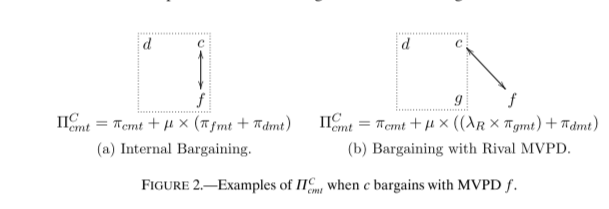
\includegraphics[height=\textheight]{figure2}
\end{frame}

\begin{frame}{5.1.3 Estimation Results using Logit:Stage 1}
    \begin{columns}[c] 
    \column{9cm}
    \begin{figure}
        \centering
        \includegraphics[height=8cm]{table2}
    \end{figure}
    \column{2cm}
    \begin{itemize}
        \item 
    \end{itemize}
	\end{columns}
\end{frame}

\begin{frame}{5.1.3 Estimation Results using Logit:Reduced-Form and Second-Stage}
    \begin{columns}[c] 
    \column{9cm}
    \begin{figure}
        \centering
        \includegraphics[height=8cm]{table3}
    \end{figure}
    \column{4cm}
    \begin{itemize}
        \item Why WTP distincts?
    \end{itemize}
	\end{columns}
\end{frame}

\begin{frame}{5.1.4 Robustness of the Estimates}
    \begin{columns}[c] 
    \column{9cm}
    \begin{figure}
        \centering
        \includegraphics[height=8cm]{table4}
    \end{figure}
    \column{4cm}
    \begin{itemize}
        \item second-stage robustness check
        \item Different bandwidth
        \item Panel A/B:local linear reg/local quadratic reg
    \end{itemize}
	\end{columns}
\end{frame}

\begin{frame}{5.1.5 Potential Confounding Factors to the Estimation}
	\textbf{}
	\begin{itemize}
	    \item Smoothness of running variable in RD design.
	    \item migration of households from north to south.\textbf{Hukou}
	    \item Other policies that use the Huai River Policy. No Chen et al. (2013)
	    \item Subsidy to heating supply in the north,   north households implicitly have higher income.
	    \item availability of HEPA between north and south.
	\end{itemize}
\end{frame}

\section{Results and Parameter Estimates}

\begin{frame}[fragile]{5.2 Random-coefficient Logit Estimation.}
      \begin{itemize}
          \item     standart logit assumes $\beta$ the preference for clean air and price $\alpha$ are indifferent across individuals, thus homogeneous MWTP $-\beta/\alpha$ across individuals.
          \item $\beta_i = \beta_0+\beta_1 y_i +\mu_i$,$\alpha = \alpha_0 +\alpha_{1}y_i+e_i$
          \item $\mu_i\rightarrow N(0,\sigma_\beta),e_i\rightarrow N(0,\sigma_\alpha)$
      \end{itemize}
\end{frame}


\begin{frame}{5.2.2 Estimation Results}
    \begin{columns}[c] 
    \column{9cm}
    \begin{figure}
        \centering
        \includegraphics[height=8cm]{Figure3}
    \end{figure}
    \column{4cm}
    \begin{itemize}
        \item 
        \item 
        \item 
    \end{itemize}
	\end{columns}
\end{frame}

\begin{frame}{5.2.2 Estimation Results}
    \begin{columns}[c] 
    \column{9cm}
    \begin{figure}
        \centering
        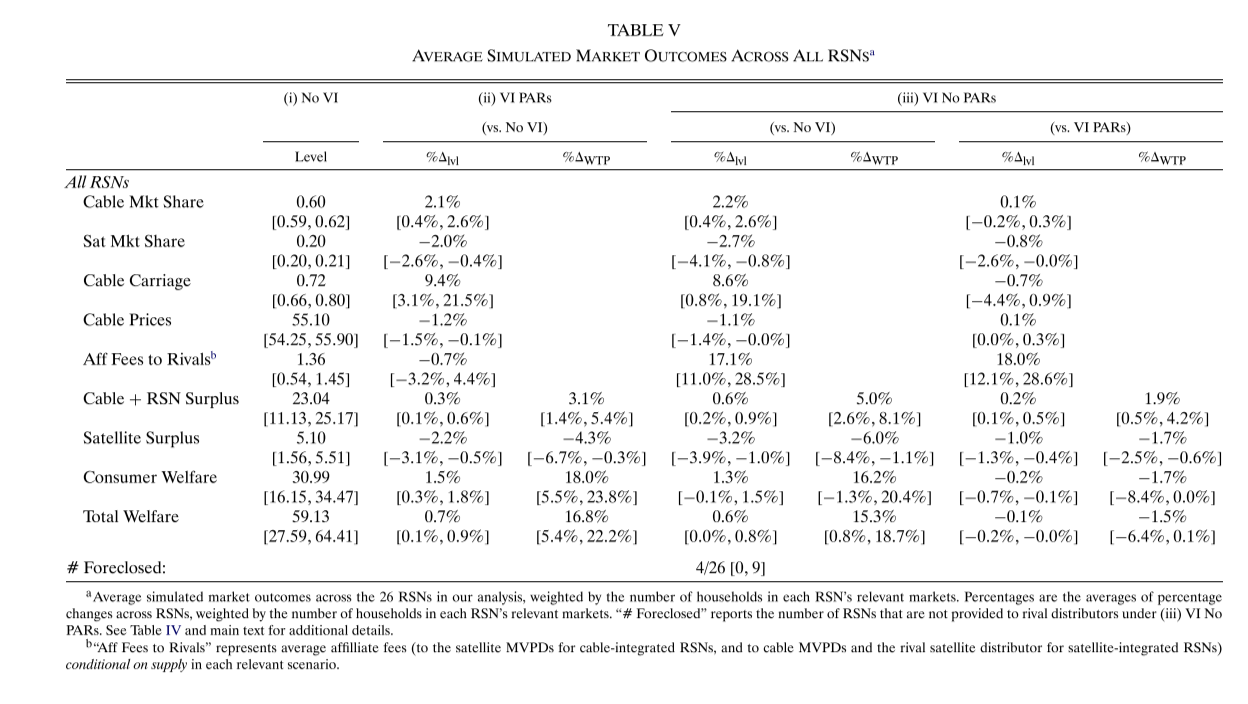
\includegraphics[height=8cm]{table5}
    \end{figure}
    \column{4cm}
    \begin{itemize}
        \item controls for latitude is different between column1,2
        \item MWTP:5.13/5.46 USD slightly larger than logit.
        \item significant $\beta_1$ means positive relationship between $y_i$ and $\beta$. but no significant relationship between $y_i$ and $\alpha$.
        \item coefficient for $\sigma_\alpha$
    \end{itemize}
	\end{columns}
\end{frame}

\begin{frame}{5.2.2 Visual Displaying Estimation Results}
    \begin{columns}[c] 
    \column{9cm}
    \begin{figure}
        \centering
        \includegraphics[height=8cm]{Figure4}
    \end{figure}
    \column{4cm}
    \begin{itemize}
        \item $mwtp_i = -(\hat{\beta_0}+\hat{\beta_1 y_i}+\mu_i)/(\hat{\alpha_0}+\hat{\alpha_1 y_i}+e_i)$
        \item wide dispersion; long right tail
        \item driven by $\beta_1 y_i$ and $e_i$
    \end{itemize}
	\end{columns}
\end{frame}
\begin{frame}{5.2.2 Visual Displaying Estimation Results}
    \begin{columns}[c] 
    \column{9cm}
    \begin{figure}
        \centering
        \includegraphics[height=8cm]{Figure5}
    \end{figure}
    \column{4cm}
    \begin{itemize}
        \item households with income larger than 15000 is dropped in the figure.
        \item increasing with income,mwtp among [0,9] with income among [0,15000].
        \item not suprisingly, the BLP indicates heterogeneity of results: higher-income vs lower-income.
    \end{itemize}
	\end{columns}
\end{frame}
\begin{frame}{Useful tips for programming of BLP}
    \item \url{https://mark-ponder.com/tutorials/static-discrete-choice-models/some-modified-blp-code/}
\end{frame}


\section{6 The Welfare Effects of Vertical Integration}
\begin{frame}{6 The Welfare Effects of Vertical Integration}
    use model's estimates to examine how vertical integration affects 1. affiliate fee (supply or not) 2.distributor's pricing and carriage decisions 3. Ultimately, firm and consumer welfare. 
    \begin{itemize}
        \item 26 RSNs active 2007, 13 integrated -10 with a cable MVPD, 3 with DirecTV
        \item CSN Phildelphia and 4SD---owned by cable distributors in "loophole" market
    \end{itemize}
\end{frame}
\begin{frame}{6 The Welfare Effects of Vertical Integration 2}
    For each of these RSNs, we simulate market outcomes for the year 2007 under "what-ifs"
    \begin{itemize}
        \item Non-integration:$\mu=0,\lambda_R=0$
        \item Integration with PARs: 
        \begin{itemize}
            \item Assign the largest cable MVPD in the relevant RSN's market
            \item $\mu=\hat{\mu}=0.79, \lambda_R=0$
        \end{itemize}
        \item Integration without PARs
        \begin{itemize}
            \item same as integration with PARs
            \item except $\lambda_R=\hat{\underline{\lambda_{R}^{Phil}}}$: larger one of two loophole market.
        \end{itemize}
    \end{itemize}
\end{frame}
\begin{frame}{6 The Welfare Effects of Vertical Integration 3}
    For each of these RSNs, we simulate market outcomes for the year 2007 under "what-ifs"
    \begin{itemize}
        \item Non-integration:$\mu=0,\lambda_R=0$
        \item Integration with PARs: 
        \begin{itemize}
            \item Assign the largest cable MVPD in the relevant RSN's market
            \item $\mu=\hat{\mu}=0.79, \lambda_R=0$
        \end{itemize}
        \item Integration without PARs
        \begin{itemize}
            \item same as integration with PARs
            \item except $\lambda_R=\hat{\underline{\lambda_{R}^{Phil}}}$: larger one of two loophole market.
        \end{itemize}
        \item each scenerio and each RSN, solve for a set of Bundle Prices, Cariage Decisions, Affiliate Fees satisfying (5), (6), (11)
        \item assume that a change in ownership for a single RSN does not change national satellite prices to adjust.
    \end{itemize}
\end{frame}
\subsection{6.1 Potential Effects}
\begin{frame}{6.1 Potential Effects1}
    Before show the counter-factual, we highlight the effects of VI captured by this model. Suppose that MVPD f integrates with RSN c, and that there is a rival MVPD g.
    \begin{itemize}
        \item Bargaining Effects and Foreclosure
        \begin{itemize}
            \item Intertal Bargaining: effective affiliate fee falls.
            \item External Bargaining: PAR in effect---RSN ignores any benefit to c from denying access from g; negotiated fee of g still affected by f's carriages and prices, and internal affiliates fee that c receives from f.
            \item Internal Bargaining: PAR not in effect: c internalize the benefit from denying g to f$\rightarrow$higher $\tau_{gct}$ or even no supply
        \end{itemize}
    \end{itemize}
\end{frame}
\begin{frame}{6.1 Potential Effects2}
    Carriage Effects: $\mu>0$ f internalize the effect that the carriage of c add to c's profit.
        \begin{itemize}
            \item direction 1:c's profit $\uparrow$ as $\tau_{fct}\uparrow$ 
            \item direction 2: c's profit $\downarrow$ as $\tau_{gct}\downarrow$ because f's carriage of c.
            \item net effect also depends on equilibrium price adjustment and whether rival distributors still carries c.
        \end{itemize}
\end{frame}
\begin{frame}{6.1 Potential Effects3}
    price effects: $\partial{P_{fmt}}/\partial{\mu}$
        \begin{itemize}
            \item direction 1:$P_{fmt}\downarrow/$ to increase f's market share,hence $\tau_{fct}\uparrow$
            \item direction 2: potential offsetting effect from $\tau_{gct}\downarrow$
            \item net effect also depends on equilibrium price adjustment and whether rival distributors still carries c.
            \item In addition, $\partial{P_{fmt}}/\partial{pr(c\in \mathcal{B}_{fmt})}$ 
        \end{itemize}
\end{frame}
\begin{frame}{6.1 Potential Effects-Sum}
    Direction not determined! Magnitude not determined! Empirical Results Needed!
\end{frame}
\subsection{6.2 Results}
\begin{frame}{6.2 Results-6.2.1 Individual RSN Results}
    \begin{columns}[c] 
    \column{9cm}
    \begin{figure}
        \centering
        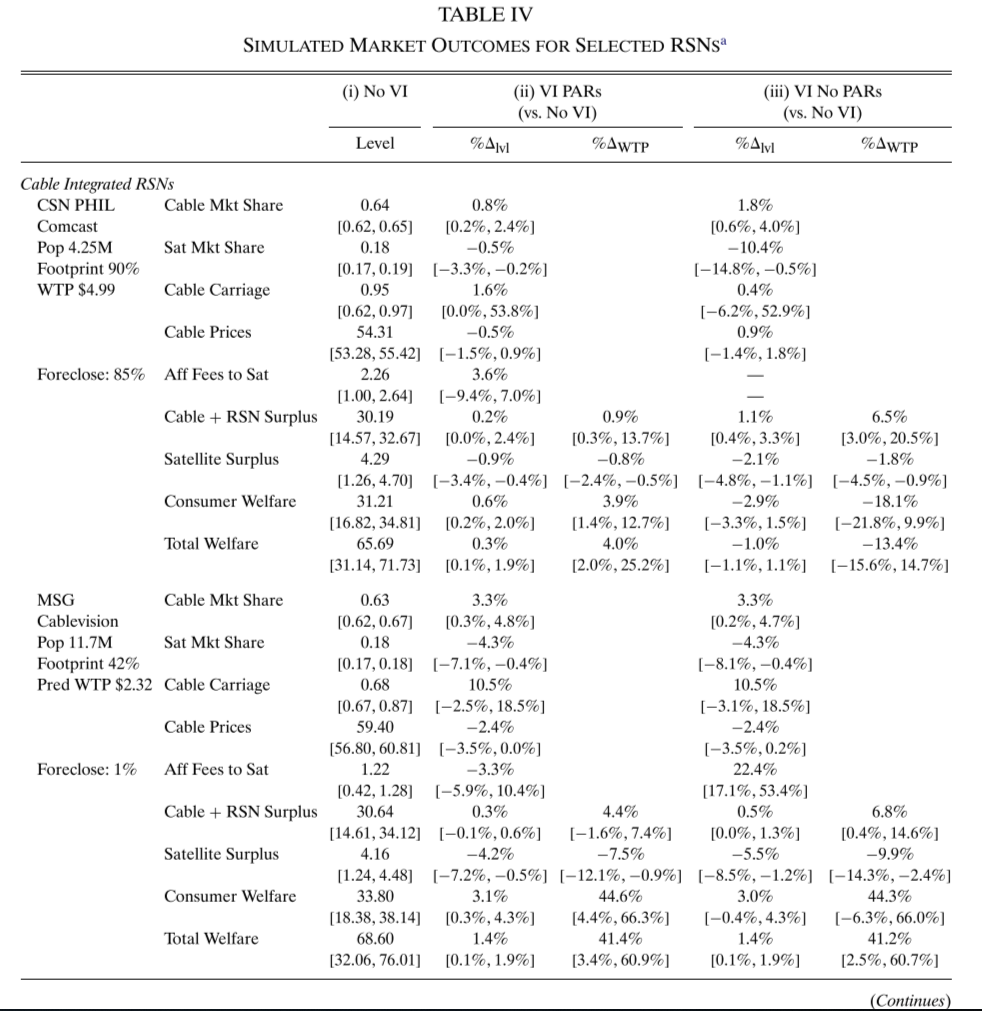
\includegraphics[height=8cm]{table4-1}
    \end{figure}
    \column{4cm}
    \begin{itemize}
        \item market share; carriage; prices;welfares
        \item 3 VI scenerios
        \item CSN Phila:cable-VI RSN in loophole market
        \item MSG:cable VI RSN non-loophole
        \item NESN: non VI RSN
    \end{itemize}
	\end{columns}
\end{frame}
\begin{frame}{6.2.1 Individual RSN Results 2}
    \begin{columns}[c] 
    \column{9cm}
    \begin{figure}
        \centering
        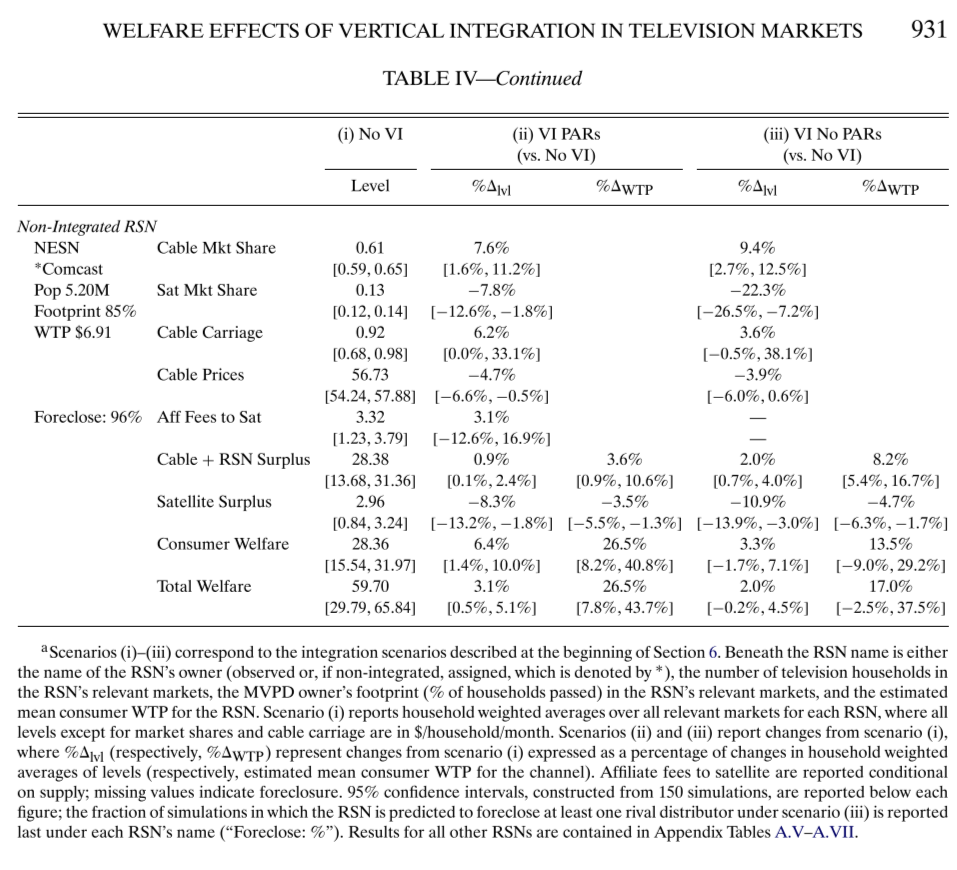
\includegraphics[height=8cm]{table4-2}
    \end{figure}
    \column{4cm}
    \begin{itemize}
        \item foreclose:the frac of simulations RSN foreclose to at least 1 rival distributor.
        \item *comcast: the name of the owner (assigned if Non-VI)
        \item CSN Phila:cable-VI RSN in loophole market
        \item MSG:cable VI RSN non-loophole
        \item NESN: non VI RSN
    \end{itemize}
	\end{columns}
\end{frame}

\begin{frame}{6.2.2 Average Results}
    \begin{figure}
        \footnotesize
        \centering
        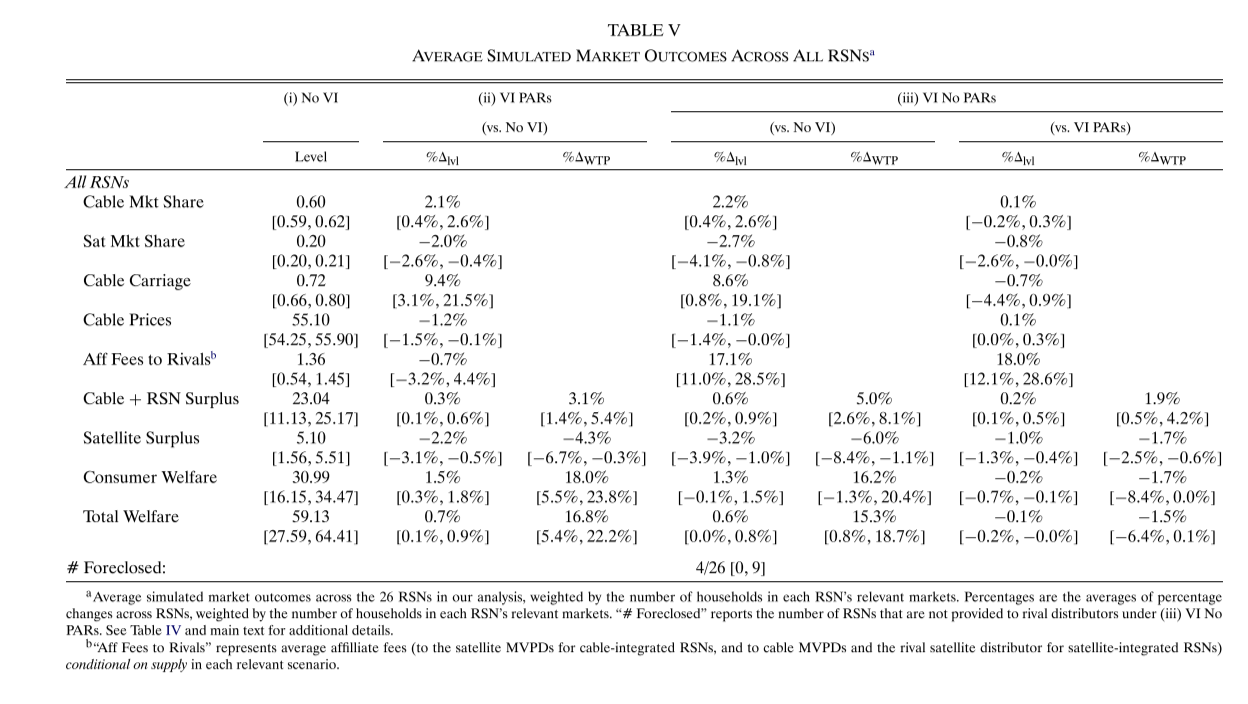
\includegraphics[height=7.2cm, width=11cm]{table5}
        \label{fig:my_label}
    \end{figure}
\end{frame}
\begin{frame}{6.2.2 Average Results:1st effect}
    \begin{itemize}
        \item Bargaining Effect and Foreclosure
        \item Efficiency effect: reduction of double marginalization and increased carriage
        \item scenerio (ii) vs (i)
        \item carriage $\uparrow$ 9.4\%, $p_{mt}\downarrow 1.2\%$, price reduction $\leftarrow$ reduction of double marginalization. 
        \item Cable+RSN surplus $\uparrow$ 0.3\%, satellite surplus $-2.2\%$
        \item consumer welfare mainly from lower cable prices: recompute the equilibrium outcome hold cable price fixed.
    \end{itemize}
\end{frame}
\begin{frame}{6.2.2 Average Results:1st effect}
    \begin{itemize}
        \item Bargaining Effect and Foreclosure
        \item Foreclosure effect: without PAR
        \item scenario (ii) vs (iii)
        \item consumer welfare and total welfare:$-0.2\%$,$-0.1\%$
        \item this results from two effects: RSN refuse to supply one rival MVPD; RSN raise the affiliate fee.
    \end{itemize}
\end{frame}
\subsection{Robustness}
\section{Conclusion Remarks}
\begin{frame}{Summary}

  Get the source of this theme and the demo presentation from

  \begin{center}\url{github.com/matze/mtheme}\end{center}

  The theme \emph{itself} is licensed under a
  \href{http://creativecommons.org/licenses/by-sa/4.0/}{Creative Commons
  Attribution-ShareAlike 4.0 International License}.

  \begin{center}\ccbysa\end{center}

\end{frame}

{\setbeamercolor{palette primary}{fg=black, bg=yellow}
\begin{frame}[standout]
  Questions?
\end{frame}
}

\appendix

\begin{frame}[fragile]{Backup slides}
  Sometimes, it is useful to add slides at the end of your presentation to
  refer to during audience questions.

  The best way to do this is to include the \verb|appendixnumberbeamer|
  package in your preamble and call \verb|\appendix| before your backup slides.

  \themename will automatically turn off slide numbering and progress bars for
  slides in the appendix.
\end{frame}

\begin{frame}[allowframebreaks]{References}

  \bibliography{demo}
  \bibliographystyle{abbrv}

\end{frame}

\end{document}

